% Date : 28/12/2022
% Version : 2
% Auteur : DDH
% Relu : 
% Relecteur : Stéphane Bargot
% Relecteur 2: Alexis Drouart

% ------------------------------------------------------------ %
% ----------------------  Fiche GAL02  ----------------------- %
% Thème : chiffres significatifs et incertitudes
% Classes : sup
% ------------------------------------------------------------ %



% ======================================================= % 
% ============== Gestion de la compilation ============== %
% ======================================================= % 
\ifdefined\mainIsLoaded\else
\RequirePackage{import}
\subimport{../../}{_preambule_CdE_PC}
\subimport{./_images/}{vernier_DDH_v2.tex}
\begin{document}
\fi

% ======================================================= % 
% ======================================================= % 






% ============================================================================ %
%                            FICHE D'ENTRAÎNEMENT                              %
% ============================================================================ %
% ======================= Métadonnées sur la fiche =========================== %
\titreFicheEntrainement		{Chiffres significatifs et incertitudes}
\grandTheme					{Généralités}
\numeroFiche				{GAL02}
\uniqueID					{WDDHInvmaq} % une chaîne de caractères (a-z, A-Z) aléatoire de 10 caractères.
\nombreColonnesReponses		{2} % 1, 2, 3, etc.
% ============================================================================ %

%%%%%%%%%%%%%%%%%%%%%%%%%%%%%%%%%%%%%%%%%%%%%%%%%%%%%%%%%%%%%%%%%%%%%%%%%%%%%%%%%%%%%%%%%%%%%%
\debutFicheEntrainement                                                                      %
%%%%%%%%%%%%%%%%%%%%%%%%%%%%%%%%%%%%%%%%%%%%%%%%%%%%%%%%%%%%%%%%%%%%%%%%%%%%%%%%%%%%%%%%%%%%%%




% --------------------------------------------------------------------- %
%                              Prérequis                                %
%                             (facultatif)                              %
% --------------------------------------------------------------------- %
% ================== Métadonnées sur le prérequis ===================== %
\avecPrerequis{Y} % Y ou N
% ===================================================================== %
\begin{prerequis}
\begin{itemize}
  \item Les incertitudes sont à donner avec deux chiffres significatifs.
  \item Toutes les incertitudes fournies sont des incertitudes-type.
\end{itemize}
	
	Ainsi, si le résultat d'une mesure de vitesse est de 30 mètres par seconde avec une incertitude-type de 1 mètre par seconde, on notera cette vitesse 
	\[
	v=\SI{30,0\pm 1,0}{\metre\per\second}.
	\]
\end{prerequis}
% --------------------------------------------------------------------- %






% •••••••••••••••••••••••••••••••••••••••••••••••••••••••••••••••••••••••••••• %
% •••••••••••••••••••••••••••••••••••••••••••••••••••••••••••••••••••••••••••• %
\sectionFicheEntrainement{Résultats numériques}
% •••••••••••••••••••••••••••••••••••••••••••••••••••••••••••••••••••••••••••• %
% •••••••••••••••••••••••••••••••••••••••••••••••••••••••••••••••••••••••••••• %



% ********************************************************************* %
%                           ENTRAÎNEMENT                                % 
% ********************************************************************* %
% ================ Métadonnées sur l'entraînement ===================== %

\titreEntrainementFacultatif	{Écriture scientifique}
\hauteurLargeurCadreReponse		{6mm}{3cm}
\dureeResolutionFacultative		{1} % 1, 2, 3 ou 4
\typeEntrainement				{Newton} % Newton ou QCM ou AN ou vide (exercice "normal")
\basiqueEtTransversal			{Y}
\nombreColonnesQuestions		{2} % vide, 1, 2, 3, etc.
\avecPlusieursQuestions			{Y} % Y ou N
\initialisationEntrainement
% ===================================================================== %

Réécrire les nombres en utilisant l'écriture scientifique. On veillera à garder les chiffres significatifs.

% =============================================================================== %
\debutEntrainement
% =============================================================================== %

% ^^^^^^^^^^^^^^^^^^^^^^^^^^^^^^^^^^^^^^ %
%               Question                 %
% ^^^^^^^^^^^^^^^^^^^^^^^^^^^^^^^^^^^^^^ %

\begin{enonce}
\num{31.5}
\end{enonce}

\reponse{\num{3.15e1}}

\begin{corrige}
Pour passer en écriture scientique, on garde une puissance de 10 et un préfacteur compris entre 1 (inclus) et 10 (exclu). On réécrit alors \num{31.5} sous la forme \num{3.15e1}.
\end{corrige}

% ************************************** %


% ^^^^^^^^^^^^^^^^^^^^^^^^^^^^^^^^^^^^^^ %
%               Question                 %
% ^^^^^^^^^^^^^^^^^^^^^^^^^^^^^^^^^^^^^^ %

\begin{enonce}
\num{0,0019}
\end{enonce}

\reponse{\num{1,9e-3}}

\begin{corrigeNewpage}
On écrit \num{0,0019}=\num{1,9e-3}.
\end{corrigeNewpage}

% ************************************** %


% ^^^^^^^^^^^^^^^^^^^^^^^^^^^^^^^^^^^^^^ %
%               Question                 %
% ^^^^^^^^^^^^^^^^^^^^^^^^^^^^^^^^^^^^^^ %

\begin{enonce}
\num{0,8120}
\end{enonce}

\reponse{\num{8,120e-1}}

\begin{corrige}
On écrit \num{0,8120}=\num{8,120e-1}.
\end{corrige}

% ************************************** %


% ^^^^^^^^^^^^^^^^^^^^^^^^^^^^^^^^^^^^^^ %
%               Question                 %
% ^^^^^^^^^^^^^^^^^^^^^^^^^^^^^^^^^^^^^^ %

\begin{enonce}
\num{1600002}
\end{enonce}

\reponse{\num{1.600002e6}}

\begin{corrige}
On écrit \num{1600002}=\num{1.600002e6}.
\end{corrige}

% ************************************** %

% ^^^^^^^^^^^^^^^^^^^^^^^^^^^^^^^^^^^^^^ %
%               Question                 %
% ^^^^^^^^^^^^^^^^^^^^^^^^^^^^^^^^^^^^^^ %

\begin{enonce}
\num{2023.9}
\end{enonce}

\reponse{\num{2.0239e3}}

\begin{corrige}
On écrit \num{2023.9}=\num{2.0239e3}.
\end{corrige}


% ************************************** %

% ^^^^^^^^^^^^^^^^^^^^^^^^^^^^^^^^^^^^^^ %
%               Question                 %
% ^^^^^^^^^^^^^^^^^^^^^^^^^^^^^^^^^^^^^^ %

\begin{enonce}
\num{7300}
\end{enonce}

\reponse{\num{7.300e3}}

\begin{corrige}
On écrit \num{7300}=\num{7.300e3}.
\end{corrige}

% ************************************** %

% ^^^^^^^^^^^^^^^^^^^^^^^^^^^^^^^^^^^^^^ %
%               Question                 %
% ^^^^^^^^^^^^^^^^^^^^^^^^^^^^^^^^^^^^^^ %

\begin{enonce}
\num{330e6}
\end{enonce}

\reponse{\num{3.30e8}}

\begin{corrige}
On écrit \num{330e6}=\num{3.30e8}.
\end{corrige}

% ************************************** %

% ^^^^^^^^^^^^^^^^^^^^^^^^^^^^^^^^^^^^^^ %
%               Question                 %
% ^^^^^^^^^^^^^^^^^^^^^^^^^^^^^^^^^^^^^^ %

\begin{enonce}
\num{70.22e-4}
\end{enonce}

\reponse{\num{7.022e-3}}

\begin{corrige}
On écrit \num{70.22e-4}=\num{7.022e-3}.
\end{corrige}

% ************************************** %


% =============================================================================== %
\finEntrainement
% =============================================================================== %




% ********************************************************************* %
%                           ENTRAÎNEMENT                                % 
% ********************************************************************* %
% ================ Métadonnées sur l'entraînement ===================== %

\pointInterrogation				{Y}
\titreEntrainementFacultatif	{Combien de chiffres significatifs}
\hauteurLargeurCadreReponse		{6mm}{1.5cm}
\dureeResolutionFacultative		{1} % 1, 2, 3 ou 4
\typeEntrainement				{Newton} % Newton ou QCM ou AN ou vide (exercice "normal")
\basiqueEtTransversal			{Y}
\nombreColonnesQuestions		{2} % vide, 1, 2, 3, etc.
\avecPlusieursQuestions			{Y} % Y ou N
\initialisationEntrainement
% ===================================================================== %

Indiquer le nombre de chiffres significatifs des grandeurs mesurées suivantes:


% =============================================================================== %
\debutEntrainement
% =============================================================================== %


% ^^^^^^^^^^^^^^^^^^^^^^^^^^^^^^^^^^^^^^ %
%               Question                 %
% ^^^^^^^^^^^^^^^^^^^^^^^^^^^^^^^^^^^^^^ %

\begin{enonce}
une intensité électrique de \SI{.39}{\ampere}.
\end{enonce}

\reponse{2}

\begin{corrige}
C'est le nombre de chiffres de \num{.39} qu'il faut regarder, il y a 2 chiffres à partir du premier non nul, le nombre de chiffres significatifs est {2}.
\end{corrige}

% ************************************** %

% ^^^^^^^^^^^^^^^^^^^^^^^^^^^^^^^^^^^^^^ %
%               Question                 %
% ^^^^^^^^^^^^^^^^^^^^^^^^^^^^^^^^^^^^^^ %

\begin{enonce}
  une tension de \SI{12,84}{\milli\volt}.
\end{enonce}

\reponse{4}

\begin{corrige}
C'est le nombre de chiffres de \num{12.84} qu'il faut regarder, il y a 4 chiffres à partir du premier non nul, le nombre de chiffres significatifs est {4}.
\end{corrige}

% ************************************** %

% ^^^^^^^^^^^^^^^^^^^^^^^^^^^^^^^^^^^^^^ %
%               Question                 %
% ^^^^^^^^^^^^^^^^^^^^^^^^^^^^^^^^^^^^^^ %

\begin{enonce}
une vitesse de \SI{12,250}{\kilo\metre\per\hour}.
\end{enonce}

\reponse{5}

\begin{corrige}
C'est le nombre de chiffres de \num{12.250} qu'il faut regarder, il y a 5 chiffres à partir du premier non nul (il faut prendre en compte le zéro final), le nombre de chiffres significatifs est {5}.
\end{corrige}

% ************************************** %

% ^^^^^^^^^^^^^^^^^^^^^^^^^^^^^^^^^^^^^^ %
%               Question                 %
% ^^^^^^^^^^^^^^^^^^^^^^^^^^^^^^^^^^^^^^ %

\begin{enonce}
une longueur de \SI{0,0020}{\metre}.
\end{enonce}

\reponse{2}

\begin{corrige}
Les zéros avant le premier chiffre non nul ne comptent pas dans le décompte des chiffres significatifs, ceux après si: le nombre de chiffres significatifs est {2}.
\end{corrige}

% ************************************** %

% =============================================================================== %
\finEntrainement
% =============================================================================== %







% ********************************************************************* %
%                           ENTRAÎNEMENT                                % 
% ********************************************************************* %
% ================ Métadonnées sur l'entraînement ===================== %

\titreEntrainementFacultatif	{Opérations et chiffres significatifs}
\hauteurLargeurCadreReponse		{6mm}{3cm}
\dureeResolutionFacultative		{1} % 1, 2, 3 ou 4
\typeEntrainement				{AN} % Newton ou QCM ou AN ou vide (exercice "normal")
\basiqueEtTransversal			{Y}
\nombreColonnesQuestions		{1} % vide, 1, 2, 3, etc.
\avecPlusieursQuestions			{Y} % Y ou N
\initialisationEntrainement
% ===================================================================== %

Effectuer les calculs en gardant le bon nombre de chiffres significatifs.

% =============================================================================== %
\debutEntrainement
% =============================================================================== %


% ^^^^^^^^^^^^^^^^^^^^^^^^^^^^^^^^^^^^^^ %
%               Question                 %
% ^^^^^^^^^^^^^^^^^^^^^^^^^^^^^^^^^^^^^^ %

\begin{enonce}
Combien de kilomètres sont parcourus en $\SI{6,0}{\minute}$ par une voiture roulant à une vitesse moyenne  $v=\SI{80}{\kilo\metre\per\hour}$?
\end{enonce}

\reponse{$\SI{8,0}{\kilo\metre}$}

\begin{corrige}
Les deux données ont deux chiffres significatifs, on garde donc deux chiffres significatifs lors de la multiplication : on a \(d=v\,t=\SI{80}{\kilo\metre\per\hour}\times\SI{0,10}{\hour}=\SI{8.0}{\kilo\metre}\).
\end{corrige}

% ************************************** %


% ^^^^^^^^^^^^^^^^^^^^^^^^^^^^^^^^^^^^^^ %
%               Question                 %
% ^^^^^^^^^^^^^^^^^^^^^^^^^^^^^^^^^^^^^^ %

\begin{enonce}
Quel est le périmètre d'un rectangle de largeur \SI{6}{\milli\metre} et de longueur \SI{15}{\centi\meter}?
\end{enonce}

\reponse{$\SI{31}{\centi\metre}$}

\begin{corrige}
Il faut additionner la longueur et la largeur puis multiplier par deux : on a
\[
p=2\times(\SI{6}{mm}+\SI{15}{cm})=\SI{31.2}{cm}.
\]
Dans la somme, la précision est limitée par la longueur (précise au centimètre près). Il faut donc arrondir au centimètre près : on écrit $p=\SI{31}{cm}$.
\end{corrige}

% ************************************** %


% =============================================================================== %
\pauseEntrainement
% =============================================================================== %


\medskip

  Le gain d'un pont diviseur de tension vaut $G=\frac{R_2}{R_1+R_2}$.
  On effectue le montage avec une résistance $R_1=\SI{0,9}{\kilo\ohm}$ et d'une résistance $R_2=\SI{100}{\ohm}$. 	
  

\minusMedskip

% =============================================================================== %
\repriseEntrainement
% =============================================================================== %



% ^^^^^^^^^^^^^^^^^^^^^^^^^^^^^^^^^^^^^^ %
%               Question                 %
% ^^^^^^^^^^^^^^^^^^^^^^^^^^^^^^^^^^^^^^ %

\begin{enonce}
Que vaut le gain $G$?
\end{enonce}

\reponse{$\num{1,0e-1}$}

\begin{corrige}
Déjà, on a $R_1+R_2=\SI{0,9}{\kilo\ohm}+\SI{100}{\ohm}=\SI{1,0}{\kilo\ohm}$, avec deux chiffres significatifs.

On calcule alors le gain par une division, en gardant le plus petit nombre de chiffres significatifs entre le numérateur (trois chiffres significatifs) et le dénominateur (deux chiffres significatifs):
\[
  G=\frac{R_2}{R_1+R_2}=\frac{\SI{100}{\ohm}}{\SI{1,0}{\kilo\ohm}}=\num{1,0e-1}.
\]
\end{corrige}

% ************************************** %

% =============================================================================== %
\finEntrainement
% =============================================================================== %







% ********************************************************************* %
%                           ENTRAÎNEMENT                                % 
% ********************************************************************* %
% ================ Métadonnées sur l'entraînement ===================== %

\titreEntrainementFacultatif	{Incertitude et chiffres significatifs}
\hauteurLargeurCadreReponse		{6mm}{1.6cm}
\dureeResolutionFacultative		{1} % 1, 2, 3 ou 4
\typeEntrainement				{QCM} % Newton ou QCM ou AN ou vide (exercice "normal")
\nombreColonnesQuestions		{1} % vide, 1, 2, 3, etc.
\avecPlusieursQuestions			{N} % Y ou N
\initialisationEntrainement
% ===================================================================== %



% =============================================================================== %
\debutEntrainement
% =============================================================================== %

% ^^^^^^^^^^^^^^^^^^^^^^^^^^^^^^^^^^^^^^ %
%               Question                 %
% ^^^^^^^^^^^^^^^^^^^^^^^^^^^^^^^^^^^^^^ %

\begin{enonce}
  Une mesure de focale donne pour résultat $f'=\SI{12.0168357}{\centi\meter}$ avec une incertitude-type de $\SI{32.3166482}{\milli\meter}$. Quel sera votre résultat numérique final?
  
    \begin{listeQCM2Colonnes}
    \item $f'=\SI{12\pm 3}{\centi\meter}$
    \item $f'=\SI{120\pm 65}{\milli\meter}$
    \item $f'=\SI{12\pm 3.2}{\centi\meter}$
    \item $f'=\SI{120\pm 33}{\milli\meter}$
    \end{listeQCM2Colonnes}
  \medskip
\end{enonce}

\reponse{\reponseC{} et \reponseD{}}

\begin{corrigeNewpage}
L'incertitude-type est exprimée dans le résultat final avec deux chiffres significatifs, avec un arrondi par valeur supérieure, ou au plus près (les deux options sont acceptées). Le résultat numérique est ensuite arrondi au niveau du dernier chiffre significatif de l'incertitude-type, donc ici au millimètre. On en déduit $f'=\SI{120\pm 33}{\milli\meter}$ ou $f'=\SI{120\pm 32}{\milli\meter}$.
\end{corrigeNewpage}

% ************************************** %

% =============================================================================== %
\finEntrainement
% =============================================================================== %






% •••••••••••••••••••••••••••••••••••••••••••••••••••••••••••••••••••••••••••• %
% •••••••••••••••••••••••••••••••••••••••••••••••••••••••••••••••••••••••••••• %
\sectionFicheEntrainement{Propagation des erreurs}
% •••••••••••••••••••••••••••••••••••••••••••••••••••••••••••••••••••••••••••• %
% •••••••••••••••••••••••••••••••••••••••••••••••••••••••••••••••••••••••••••• %
\bigskip

\begin{prerequis}
On considère deux grandeurs expérimentales indépendantes $x$ et $y$, et $z=f(x,y)$ une grandeur calculée. 
\smallskip

L'incertitude-type $\incertitude(z)$ est reliée à celles de $x$ et $y$ \emph{via} les relations:
$$
\begin{array}{ccccc}
\incertitude(z)^2		
&=&a^2\incertitude^2(x)+b^2\incertitude^2(y)		
&\text{si}		
&z=ax+by	\\[3mm]

\left(\dfrac{\incertitude(z)}{z}\right)^2
&=&a^2\left(\dfrac{\incertitude(x)}{x}\right)^2+b^2\left(\dfrac{\incertitude(y)}{y}\right)^2	
&\text{si}	
&z=c\,x^ay^b
\end{array}
$$
où $a$, $b$  et $c$ sont des paramètres fixés.
\end{prerequis}



% ********************************************************************* %
%                           ENTRAÎNEMENT                                % 
% ********************************************************************* %
% ================ Métadonnées sur l'entraînement ===================== %

\titreEntrainementFacultatif	{Pour commencer}
\hauteurLargeurCadreReponse		{6mm}{2.5cm}
\dureeResolutionFacultative		{3} % 1, 2, 3 ou 4
\typeEntrainement 				{AN}% Newton ou QCM ou AN ou vide (exercice "normal")
\nombreColonnesQuestions		{1} % vide, 1, 2, 3, etc.
\avecPlusieursQuestions			{Y} % Y ou N
\initialisationEntrainement
% ===================================================================== %


On mesure $x=\SI{10.0\pm0.2}{m}$ et $y=\SI{9.1\pm0.3}{m}$. 
\smallskip

Calculer : 

% =============================================================================== %
\debutEntrainement
% =============================================================================== %

% ^^^^^^^^^^^^^^^^^^^^^^^^^^^^^^^^^^^^^^ %
%               Question                 %
% ^^^^^^^^^^^^^^^^^^^^^^^^^^^^^^^^^^^^^^ %

\begin{enonce}
$x+y$
\end{enonce}

\reponse{\SI{19.10\pm0.36}{m}}

\begin{corrige}
On a $z=x+y=\SI{19.1}{m}$ et $\incertitude(z)=\sqrt{\num{.2}^2+\num{.3}^2}=\SI{.36}{m}$. En arrondissant l'incertitude à deux chiffres, on obtient $\SI{19.10\pm0.36}{m}$.
\end{corrige}

% ************************************** %

% ^^^^^^^^^^^^^^^^^^^^^^^^^^^^^^^^^^^^^^ %
%               Question                 %
% ^^^^^^^^^^^^^^^^^^^^^^^^^^^^^^^^^^^^^^ %

\begin{enonce}
$x-y$
\end{enonce}

\reponse{\SI{.90\pm0.36}{m}}

\begin{corrige}
On a $z=x-y=\SI{.9}{m}$ et $\incertitude(z)=\sqrt{\num{.2}^2+\num{.3}^2}=\SI{.36}{m}$. En arrondissant l'incertitude à deux chiffres, on obtient \SI{.90\pm0.36}{m}.
		
{\itshape Lorsque l'on soustrait deux grandeurs physiques proches, le résultat est en général moins précis que la donnée la moins précise.}
\end{corrige}

% ************************************** %

% ^^^^^^^^^^^^^^^^^^^^^^^^^^^^^^^^^^^^^^ %
%               Question                 %
% ^^^^^^^^^^^^^^^^^^^^^^^^^^^^^^^^^^^^^^ %

\begin{enonce}
$x\times y$
\end{enonce}

\reponse{\SI{91.0\pm3.5}{m^2}}

\begin{corrige}
On a $z=x\times y=\SI{91}{m^2}$ et $\incertitude(z)=91\times \sqrt{(\num{.2}/10)^2+(\num{.3}/\num{9.1})^2}=\SI{3.51}{m^2}$. En arrondissant l'incertitude à deux chiffres, on obtient \SI{91.0\pm3.5}{m^2}.
\end{corrige}

% ************************************** %

% ^^^^^^^^^^^^^^^^^^^^^^^^^^^^^^^^^^^^^^ %
%               Question                 %
% ^^^^^^^^^^^^^^^^^^^^^^^^^^^^^^^^^^^^^^ %

\begin{enonce}
$\frac{y}{x}$
\end{enonce}

\reponse{\num{.910\pm .035}}

\begin{corrige}
On a $z=y/x=\num{.91}$ et $\incertitude(z)=\num{.91}\times \sqrt{(\num{.2}/10)^2+(\num{.3}/\num{9.1})^2}=\num{.0351}$. En arrondissant l'incertitude à deux chiffres, on obtient (\num{9.10\pm.35})$\times 10^{-1}$.
\end{corrige}

% ************************************** %

% =============================================================================== %
\finEntrainement
% =============================================================================== %



% ********************************************************************* %
%                           ENTRAÎNEMENT                                % 
% ********************************************************************* %
% ================ Métadonnées sur l'entraînement ===================== %


\titreEntrainementFacultatif	{Dosage d'une solution}
\hauteurLargeurCadreReponse		{6mm}{3cm}
\dureeResolutionFacultative		{2} % 1, 2, 3 ou 4
\typeEntrainement 				{AN}% Newton ou QCM ou AN ou vide (exercice "normal")
\basiqueEtTransversal			{Y}
\nombreColonnesQuestions		{1} % vide, 1, 2, 3, etc.
\avecPlusieursQuestions			{N} % Y ou N
\initialisationEntrainement
% ===================================================================== %


% ===================================================================== %
\debutEntrainement
% ===================================================================== %

On dose une solution acide de concentration $c_A$ inconnue. Le volume de solution dosée est $V_A$, et la solution utilisée pour le dosage est de concentration $c_B$. À l'équivalence, un volume $V_B$ de base est versée et l'on a 
\[
  c_A=\frac{c_B\times V_B}{V_A}
\]
La base est préparée de sorte à avoir \( c_B = \SI{100.0\pm 2.0}{\milli\mole\per\liter} \). 

De plus, on mesure les volumes \( V_A = \SI{20,00\pm 0,10}{\milli\liter} \) et \( V_B = \SI{11.80\pm 0,10}{\milli\liter} \)


% ^^^^^^^^^^^^^^^^^^^^^^^^^^^^^^^^^^^^^^ %
%               Question                 %
% ^^^^^^^^^^^^^^^^^^^^^^^^^^^^^^^^^^^^^^ %

\begin{enonce}
  Quel résultat obtient-on pour $c_A$? (en \si{\milli\mol\per\liter})
\end{enonce}

\reponse{\SI{59.0 \pm 1.4}{\milli\mol\per\liter}}

\begin{corrige}
  On commence par calculer le résultat avant de s'intéresser aux incertitudes:
  \[
     c_A=\frac{c_B\cdot V_B}{V_A}= \frac{\SI{100.0}{\milli\mole\per\liter}\cdot \SI{11.8}{\milli\liter}}{\SI{20}{\milli\liter}} = \SI{59}{\milli\mole\per\liter}.
  \]
  On propage l'incertitude pour ce produit de grandeurs indépendantes:
  \[
    \frac{\incertitude(c_A)}{c_A}=\sqrt{\left(\frac{\incertitude(c_B)}{c_B}\right)^2 + \left(\frac{\incertitude(V_A)}{V_A}\right)^2 + \left(\frac{\incertitude(V_B)}{V_B}\right)^2 }.
  \]
  Numériquement, cela donne
  \[
    {\incertitude(c_A)}={\SI{59}{\milli\mole\per\liter}}\sqrt{\left(\frac{\SI{2.0}{\milli\mole\per\liter}}{\SI{100.0}{\milli\mole\per\liter}}\right)^2 + \left(\frac{\SI{0,10}{\milli\liter}}{\SI{20,00}{\milli\liter}}\right)^2 + \left(\frac{\SI{ 0,10}{\milli\liter}}{\SI{11.80}{\milli\liter}}\right)^2 }.
  \]
  On obtient \( {\incertitude(c_A)} = \SI{1.4}{\milli\mol\per\liter} \), et finalement \( c_A=\SI{59.0 \pm 1.4}{\milli\mol\per\liter} \).
\end{corrige}

% ************************************** %


% ===================================================================== %
\finEntrainement
% ===================================================================== %



\newpage



% ********************************************************************* %
%                           ENTRAÎNEMENT                                % 
% ********************************************************************* %
% ================ Métadonnées sur l'entraînement ===================== %

\titreEntrainementFacultatif	{Puissance électrique dans une résistance}
\hauteurLargeurCadreReponse		{6mm}{3cm}
\dureeResolutionFacultative		{2} % 1, 2, 3 ou 4
\typeEntrainement 				{AN}% Newton ou QCM ou AN ou vide (exercice "normal")
\basiqueEtTransversal			{Y}
\nombreColonnesQuestions		{1} % vide, 1, 2, 3, etc.
\avecPlusieursQuestions			{Y} % Y ou N
\initialisationEntrainement
% ===================================================================== %


% ===================================================================== %
\debutEntrainement
% ===================================================================== %

On désire mesurer la puissance dissipée par effet Joule dans une résistance, donnée par  \( \mathcal P = U\times I  = R\,I^2 \).

Donner la puissance (exprimée en watts) et son incertitude pour les mesures suivantes :

% ^^^^^^^^^^^^^^^^^^^^^^^^^^^^^^^^^^^^^^ %
%               Question                 %
% ^^^^^^^^^^^^^^^^^^^^^^^^^^^^^^^^^^^^^^ %

\begin{enonce}
  \( U= \SI{2,382\pm 0,050}{\volt} \) \quad et \quad\( I= \SI{0,500\pm 0,010}{\ampere} \) 
\end{enonce}

\reponse{\SI{1,191\pm 0,035}{\watt}}

\begin{corrige}
On calcule la puissance : \( \mathcal P = U\times I = \SI{2,382}{\volt} \times \SI{0,500}{\ampere}= \SI{1,191}{\watt}\).
  
On applique ici la propagation des incertitudes à \( \mathcal P = U\times I \),
\[
\frac{\incertitude(\mathcal P)}{\mathcal P}=\sqrt{\left(\frac{\incertitude(U)}{U}\right)^2 + \left(\frac{\incertitude(I)}{I}\right)^2}.
\]
  Numériquement, cela donne 
\[
\incertitude(\mathcal P)=\SI{1,202}{\watt} \times \sqrt{\left(\frac{\SI{0,050}{\volt}}{\SI{2,382}{\volt}}\right)^2 + \left(\frac{\SI{ 0,010}{\ampere}}{\SI{0,500}{\ampere}}\right)^2}=\SI{.035}{\watt}.
  \]
  Finalement, on obtient \( \mathcal P =  \SI{1,191\pm0,035}{\watt} \).
\end{corrige}

% ************************************** %


% ^^^^^^^^^^^^^^^^^^^^^^^^^^^^^^^^^^^^^^ %
%               Question                 %
% ^^^^^^^^^^^^^^^^^^^^^^^^^^^^^^^^^^^^^^ %

\begin{enonce}
  \( I= \SI{0,500\pm 0,010}{\ampere} \) \quad et \quad  \(R=\SI{4,7\pm.14}{\ohm}\)
\end{enonce}

\reponse{\SI{1,175\pm 0,059}{\watt}}

\begin{corrige}
  On calcule la puissance :  \( \mathcal P = R\times I^2 = \SI{4,7}{\ohm} \times (\SI{0,500}{\ampere})^2= \SI{1,175}{\watt}\).
  
  On applique ici la propagation des incertitudes à \( \mathcal P = R\times I^2 \) : on a
  \[
    \frac{\incertitude(\mathcal P)}{\mathcal P}=\sqrt{\left(\frac{\incertitude(R)}{R}\right)^2 + 2^2\left(\frac{\incertitude(I)}{I}\right)^2}.
  \]
Numériquement, cela donne \minusMedskip
\[
\incertitude(\mathcal P)=
\SI{1,175}{\watt}\sqrt{
\left(\frac{\num{.14}}{100}\right)^2 + 
4\times\left(\frac{\SI{ 0,010}{\ampere}}{\SI{0,500}{\ampere}}\right)^2
}=\SI{0,059}{\watt}.
\]
Finalement, on obtient \( \mathcal P =  \SI{1,175\pm0,059}{\watt} \).
\end{corrige}

% ************************************** %

% ^^^^^^^^^^^^^^^^^^^^^^^^^^^^^^^^^^^^^^ %
%               Question                 %
% ^^^^^^^^^^^^^^^^^^^^^^^^^^^^^^^^^^^^^^ %

\begin{enonce}
Ces deux mesures sont-elles compatibles ?
% Les données précédentes sont-elles cohérentes avec un unique montage?
   \begin{listeQCM2Colonnes}
     \item Oui
     \item Non
   \end{listeQCM2Colonnes}
   \smallskip
\end{enonce}

\reponse{\reponseA{}}

\begin{corrige}
  Les mesures sont \( \mathcal P = \SI{1,191\pm 0,035}{\watt} \) et \( \mathcal P =  \SI{1,175\pm0,059}{\watt} \). Les deux intervalles se recoupent : les mesures sont compatibles.
\end{corrige}

% ************************************** %

% ===================================================================== %
\finEntrainement
% ===================================================================== %





% ********************************************************************* %
%                           ENTRAÎNEMENT                                % 
% ********************************************************************* %
% ================ Métadonnées sur l'entraînement ===================== %


\titreEntrainementFacultatif	{Diamètre d'un tube}
\hauteurLargeurCadreReponse		{6mm}{1.2cm}
\dureeResolutionFacultative		{2} % 1, 2, 3 ou 4
\typeEntrainement 				{QCM}% Newton ou QCM ou AN ou vide (exercice "normal")
\basiqueEtTransversal			{Y}
\nombreColonnesQuestions		{1} % vide, 1, 2, 3, etc.
\avecPlusieursQuestions			{Y} % Y ou N
\initialisationEntrainement
% ===================================================================== %

% ===================================================================== %
\debutEntrainement
% ===================================================================== %


On mesure l'épaisseur d'un tube cylindrique au pied à coulisse. 

Le diamètre intérieur du tube est $d = \SI{6,8\pm .1}{\milli\metre}$ et le diamètre extérieur $D= \SI{10.3\pm .1}{\milli\metre}$.

% ^^^^^^^^^^^^^^^^^^^^^^^^^^^^^^^^^^^^^^ %
%               Question                 %
% ^^^^^^^^^^^^^^^^^^^^^^^^^^^^^^^^^^^^^^ %

\begin{enonce}
  Exprimer l'épaisseur $e$ du tube en fonction de $d$ et $D$.
  \smallskip
  
  \begin{listeQCM4Colonnes}
    \item \(\pi (D^2 -d^2 ) \)
    \item \(\frac{D-d}{2} \)
    \item \(\sqrt{ D^2 +d^2 } \)
    \item \(\frac{d-D}{2} \)
  \end{listeQCM4Colonnes}
  \smallskip
\end{enonce}

\reponse{\reponseB{}}

\begin{corrige}
  L'épaisseur du tube est la différence entre le rayon du cylindre extérieur et le rayon intérieur. Le rayon étant la moitié du diamètre, on trouve \(e=\frac{D}{2}- \frac{d}{2}\).
\end{corrige}

% ************************************** %

% ^^^^^^^^^^^^^^^^^^^^^^^^^^^^^^^^^^^^^^ %
%               Question                 %
% ^^^^^^^^^^^^^^^^^^^^^^^^^^^^^^^^^^^^^^ %

\begin{enonce}
  En déduire l'expression de l'incertitude-type sur l'épaisseur $\incertitude(e)$ en fonction de \( D \), \( d \), \(\incertitude(d)\) et \(\incertitude(D)\).
  \smallskip
  
  \begin{listeQCM2Colonnes}
    \item  \( \frac12 \sqrt{\incertitude^2(D) + \incertitude^2(d) }\)\medskip
    \item \(  \sqrt{\left(\frac{\incertitude(D)}{D}\right)^2  + \left(\frac{\incertitude(d)}{d}\right)^2  }\)
    \item \(  \sqrt{u^2(D) + u^2(d) }\) \medskip
    \item \(  \frac12 \sqrt{\left(\frac{\incertitude(D)}{D}\right)^2  + \left(\frac{\incertitude(d)}{d}\right)^2  }\)
  \end{listeQCM2Colonnes}
  \smallskip
\end{enonce}

\reponse{ \reponseA{}}

\begin{corrige}
On applique la formule donnée dans les prérequis de cette section avec $a=\frac12$ et $b=-\frac12$. On trouve \vspace{-1mm}
\[
\incertitude(e)= \sqrt{ 
\left( \frac12 \right)^2 \incertitude^2(D)+\left(-\frac12\right)^2 \incertitude^2(d)
}
=\frac12 \sqrt{\incertitude^2(D) + \incertitude^2(d) }.
\]
\end{corrige}

% ************************************** %

% ^^^^^^^^^^^^^^^^^^^^^^^^^^^^^^^^^^^^^^ %
%               Question                 %
% ^^^^^^^^^^^^^^^^^^^^^^^^^^^^^^^^^^^^^^ %

\begin{enonce}
En déduire le résultat de la mesure de \(e\).
\begin{listeQCM2Colonnes}
    \item \(e= \SI{1.75 \pm 0,07}{\milli\metre}\)
    \item \(e= \SI{1.75 \pm 0,10}{\milli\metre}\)
    \item \(e= \SI{1.8 \pm 0,1}{\milli\metre} \)
    \item \(e= \SI{1.750 \pm 0,071}{\milli\metre} \)
\end{listeQCM2Colonnes}
\smallskip
\end{enonce}

\reponse{\reponseD{}}

\begin{corrige}
On a \( e =  \frac{\SI{10,3}{\milli\metre}-\SI{6,8}{\milli\metre}}{2} = \SI{1.75}{\milli\metre} \), et \(\incertitude(e)= \frac12 \sqrt{(\SI{.1}{\milli\metre})^2 + (\SI{.1}{\milli\metre})^2 } = \SI{0,071}{\milli\metre} \). Finalement, on a donc \(e=\SI{1.750 \pm 0,071}{\milli\metre}\).
\end{corrige}

% ************************************** %

% ===================================================================== %
\finEntrainement
% ===================================================================== %





% ********************************************************************* %
%                           ENTRAÎNEMENT                                % 
% ********************************************************************* %
% ================ Métadonnées sur l'entraînement ===================== %

\titreEntrainementFacultatif	{Analyse d'une figure de diffraction}
\hauteurLargeurCadreReponse		{7mm}{7cm}
\dureeResolutionFacultative		{2} % 1, 2, 3 ou 4
\typeEntrainement 				{AN}% Newton ou QCM ou AN ou vide (exercice "normal")
\basiqueEtTransversal			{Y}
\nombreColonnesQuestions		{1} % vide, 1, 2, 3, etc.
\avecPlusieursQuestions			{Y} % Y ou N
\initialisationEntrainement
% ===================================================================== %


% ===================================================================== %
\debutEntrainement
% ===================================================================== %

On mesure la figure de diffraction obtenue en interposant un cheveu entre un écran et un laser.
La distance entre le cheveu et l'écran est $D=(3 \pm 10 \times 10^{-3} )\,\si{m}$
%\( D = \SI{3\pm 1e-3}{\metre} \),
 la longueur d'onde du laser \( \lambda= \SI{632,80 \pm .10}{\nano\metre}  \), et l'on observe une tache de diffraction de largeur \(\ell=\SI{5,10\pm 0,30}{\centi\metre} \).

Le diamètre $d$ du cheveu peut alors se déduire de ces mesures \emph{via} la relation:
\[
  d=2\frac{\lambda\,D}{\ell}.
\]


% ^^^^^^^^^^^^^^^^^^^^^^^^^^^^^^^^^^^^^^ %
%               Question                 %
% ^^^^^^^^^^^^^^^^^^^^^^^^^^^^^^^^^^^^^^ %

\begin{enonce}
Exprimer l'incertitude $\incertitude(d)$ en fonction de $d$, $\lambda$, $D$, $\ell$, \minusSmallskip \\ et de $\incertitude(\lambda)$, $\incertitude(D)$ et $\incertitude(\ell)$
\end{enonce}

\reponse{\small$%\incertitude(d)= 
d 
\sqrt{
\left(\frac{\incertitude(\lambda)}{\lambda}\right)^2 +
\left(\frac{\incertitude(D)}{D}\right)^2 +
\left(\frac{\incertitude(\ell)}{\ell}\right)^2}$}

\begin{corrige}
On a, pour ce produit de grandeurs indépendantes : \vspace{-2mm}
\[
\frac{\incertitude(d)}{d}=
\sqrt{
\left(\frac{\incertitude(\lambda)}{\lambda}\right)^2 +
\left(\frac{\incertitude(D)}{D}\right)^2 +
\left(\frac{\incertitude(\ell)}{\ell}\right)^2 }.
\]
\end{corrige}

% ************************************** %


% ^^^^^^^^^^^^^^^^^^^^^^^^^^^^^^^^^^^^^^ %
%               Question                 %
% ^^^^^^^^^^^^^^^^^^^^^^^^^^^^^^^^^^^^^^ %

\begin{enonce}
Quel résultat obtient-on pour $d$? (en \si{\micro\metre})
\end{enonce}

\reponse{\SI{74.4 \pm 4.4}{\micro\metre}}

\begin{corrige}
On commence par calculer le résultat avant de s'intéresser aux incertitudes:
\[
d=2\frac{\lambda\,D}{\ell}= 
2\times\frac{\SI{632,8}{\nano\metre}\times\SI{3}{\metre}}{\SI{51}{\milli\metre}}=\SI{74,447}{\micro\metre}.
\]
Le nombre de chiffres conservés ici n'est pas significatif, juste assez grand pour pouvoir être ajusté ensuite. On calcule ensuite numériquement l'incertitude :
\[
\incertitude(d)=
\SI{74,447}{\nano\metre} \times\sqrt{
\left(\frac{\SI{.10}{\nano\metre}}{\SI{632,8}{\nano\metre}}\right)^2 +
\left(\frac{\SI{ 10e-3}{\metre}}{\SI{3,000}{\metre}}\right)^2 + \left(\frac{\SI{ 0,30}{\centi\metre}}{\SI{5,1}{\centi\metre}}\right)^2 }
= \SI{4.4}{\micro\metre}. 
\]
Finalement, on obtient \( d =\SI{74.4 \pm 4.4}{\micro\metre} \).
\end{corrige}

% ************************************** %


% ===================================================================== %
\finEntrainement
% ===================================================================== %



\newpage



% •••••••••••••••••••••••••••••••••••••••••••••••••••••••••••••••••••••••••••• %
% •••••••••••••••••••••••••••••••••••••••••••••••••••••••••••••••••••••••••••• %
\sectionFicheEntrainement{Incertitudes expérimentales}
% •••••••••••••••••••••••••••••••••••••••••••••••••••••••••••••••••••••••••••• %
% •••••••••••••••••••••••••••••••••••••••••••••••••••••••••••••••••••••••••••• %



% ********************************************************************* %
%                           ENTRAÎNEMENT                                % 
% ********************************************************************* %
% ================ Métadonnées sur l'entraînement ===================== %

\titreEntrainementFacultatif	{Série de mesures}
\hauteurLargeurCadreReponse		{7mm}{4cm}
\dureeResolutionFacultative		{2} % 1, 2, 3 ou 4
\typeEntrainement 				{AN}% Newton ou QCM ou AN ou vide (exercice "normal")
\nombreColonnesQuestions		{1} % vide, 1, 2, 3, etc.
\avecPlusieursQuestions			{Y} % Y ou N
\initialisationEntrainement
% ===================================================================== %



% =============================================================================== %
\debutEntrainement
% =============================================================================== %

On procède à $n=10$ mesures d'une tension. Le tableau ci-dessous recense les résultats:
\begin{center}
\renewcommand{\arraystretch}{1.2}
\begin{tabular}{|r|*{10}{c}|}
\hline
\textbf{Mesure \no{}} &1&2&3&4&5&6&7&8&9&10\\
\hline
$U_i$ (en \si{\volt})&     \num{4,955}&	\num{5,596}&	\num{4,271}&	\num{4,955}&	\num{5,164}&	\num{5,371}&	\num{4,671}&	\num{4,736}&	\num{5,393}&	\num{4,183}\\
\hline
\end{tabular}
\renewcommand{\arraystretch}{1}
\end{center}

% ^^^^^^^^^^^^^^^^^^^^^^^^^^^^^^^^^^^^^^ %
%               Question                 %
% ^^^^^^^^^^^^^^^^^^^^^^^^^^^^^^^^^^^^^^ %

\begin{enonce}
Que vaut la moyenne arithmétique $m=\frac{1}{n}\sum_i U_i$ de la série?
\end{enonce}

\reponse{\SI{4,9295}{\volt}}

\begin{corrige}
On peut faire le calcul à l'aide d'un tableur (fonction \texttt{MOYENNE()} souvent), d'une calculatrice ou de python (fonction \texttt{mean()} de la bibliothèque \texttt{numpy} par exemple). On obtient $m=\sum_{i=1}^{10}U_i=\SI{4,9295}{\volt}$.
\end{corrige}

% ************************************** %

\minusMedskip

% ^^^^^^^^^^^^^^^^^^^^^^^^^^^^^^^^^^^^^^ %
%               Question                 %
% ^^^^^^^^^^^^^^^^^^^^^^^^^^^^^^^^^^^^^^ %

\begin{enonce}
Calculer l'écart-type expérimental de la série $\sigma_U=\sqrt{\frac{\sum_i(U_i-m)^2}{n-1}}$
\end{enonce}

\reponse{\SI{0.472}{\volt}}

\begin{corrige}
 Le calcul est fait par une fonction prédéfinie du tableur (\texttt{ECARTYPE()} souvent), de la calculatrice ou de python (fonction \texttt{std()} de la bibliothèque \texttt{numpy} par exemple). On obtient $\sigma_U=\SI{0,472042429825493
}{\volt}$, soit \SI{0.472}{\volt} en gardant trois chiffres significatifs.
\end{corrige}

% ************************************** %

% =============================================================================== %
\pauseEntrainement
% =============================================================================== %

\smallskip
L'incertitude-type de $m$ est donnée par $\incertitude(m)=\frac{\sigma_U}{\sqrt{n}}$. 
\minusBigskip

% =============================================================================== %
\repriseEntrainement
% =============================================================================== %




% ^^^^^^^^^^^^^^^^^^^^^^^^^^^^^^^^^^^^^^ %
%               Question                 %
% ^^^^^^^^^^^^^^^^^^^^^^^^^^^^^^^^^^^^^^ %

\begin{enonce}
En déduire le résultat final de la mesure
\end{enonce}

\reponse{\SI{4,93 \pm 0,15}{\volt}}

\begin{corrige}
On obtient alors $\incertitude(m)=\frac{\num{.472}}{\sqrt{10}}=\SI{0,149}{\volt}$, que l'on arrondit en gardant deux chiffres significatifs. 

L'incertitude-type sur la valeur moyenne est donc finalement \(\incertitude(m)=\SI{0,15}{\volt}\).

 Il faut exprimer la moyenne au centième de volt ce qui donne le résultat suivant:
 $m=\SI{4,93 \pm 0,15}{\volt}$. Cette valeur moyenne est la meilleure estimation de la \og{}valeur vraie\fg{} que l'on peut faire à partir de cette série de mesures répétées.
\end{corrige}

% ************************************** %

% =============================================================================== %
\finEntrainement
% =============================================================================== %




% ********************************************************************* %
%                           ENTRAÎNEMENT                                % 
% ********************************************************************* %
% ================ Métadonnées sur l'entraînement ===================== %

\titreEntrainementFacultatif	{Focométrie}
\hauteurLargeurCadreReponse		{7mm}{3cm}
\dureeResolutionFacultative		{2} % 1, 2, 3 ou 4
\typeEntrainement 				{AN}% Newton ou QCM ou AN ou vide (exercice "normal")
\nombreColonnesQuestions		{1} % vide, 1, 2, 3, etc.
\avecPlusieursQuestions			{N} % Y ou N
\initialisationEntrainement
% ===================================================================== %



% =============================================================================== %
\debutEntrainement
% =============================================================================== %


On procède à des mesures d'une distance focale (notée $f'$) ; le tableau ci-dessous recense les résultats:

\begin{center}
\renewcommand{\arraystretch}{1.2}
\begin{tabular}{|r|*{12}{c}|}
\hline
 $f'$ (en \si{\centi\metre})&   \num{24,6}&	\num{24,5}&	\num{25,1}&	\num{25,1}&	\num{25,3}&	\num{25,4}&	\num{24,9}&	\num{24,8}&	\num{24,9}&	\num{25,4}&	\num{25,3}&	\num{24,9}\\
\hline
\end{tabular}
\renewcommand{\arraystretch}{1}
\end{center}


\minusSmallskip

% ^^^^^^^^^^^^^^^^^^^^^^^^^^^^^^^^^^^^^^ %
%               Question                 %
% ^^^^^^^^^^^^^^^^^^^^^^^^^^^^^^^^^^^^^^ %

\begin{enonce}
Donner le résultat final de la mesure
\end{enonce}

\reponse{\SI{25.017 \pm 0,092}{\centi\metre}}

\begin{corrige}
On calcule  une valeur moyenne de \SI{25.017}{\centi\meter} et un écart-type des mesures de \SI{0.301}{\centi\metre}, ce qui donne une incertitude-type sur la valeur moyenne de \SI{0,087}{\centi\metre}. 

L'incertitude-type est, avec deux chiffres significatifs, au centième de millimètre, il faut donc garder les chiffres jusqu'à cette décimale: on obtient \SI{25.017 \pm 0,087}{\centi\metre}.
\end{corrige}

% ************************************** %

% =============================================================================== %
\finEntrainement
% =============================================================================== %






% ********************************************************************* %
%                           ENTRAÎNEMENT                                % 
% ********************************************************************* %
% ================ Métadonnées sur l'entraînement ===================== %


\titreEntrainementFacultatif	{Résistances en série}
\hauteurLargeurCadreReponse		{6mm}{1.5cm}
\dureeResolutionFacultative		{2} % 1, 2, 3 ou 4
\typeEntrainement 				{QCM}% Newton ou QCM ou AN ou vide (exercice "normal")
\nombreColonnesQuestions		{1} % vide, 1, 2, 3, etc.
\avecPlusieursQuestions			{N} % Y ou N
\initialisationEntrainement

On dispose de $n$~résistances identiques, dont l'incertitude relative est donnée à \SI{1}{\percent}. On les monte en série. Ainsi, la résistance totale est égale à la somme des résistances individuelles.

% =============================================================================== %
\debutEntrainement
% =============================================================================== %

% ^^^^^^^^^^^^^^^^^^^^^^^^^^^^^^^^^^^^^^ %
%               Question                 %
% ^^^^^^^^^^^^^^^^^^^^^^^^^^^^^^^^^^^^^^ %

\begin{enonce}
  Quelle est  l'incertitude relative pour la résistance totale lorsque $n=5$ ?
	
	\begin{listeQCM3Colonnes}
    \item $\SI{0,44}{\percent}$
	\item $\SI{1}{\percent}$
	\item $\SI{2,2}{\percent}$
	\end{listeQCM3Colonnes}

\end{enonce}

\reponse{\reponseA{}}

\begin{corrige}
 Pour une résistance, on a \( \incertitude(r) = r \times \frac{\incertitude(r)}{r} \). 
 
 Pour les $n=5$ résistances, on a \(R=n\, r\), et \(\incertitude(R)=\sqrt{ n \, u^2(r) }\), donc 
 \[
  \frac{\incertitude(R)}{R}=\frac{\sqrt{n}}{n} = \frac{1}{\sqrt{n}}.
  \]
  Pour $n=5$, on obtient \( \frac{\incertitude(R)}{R}  \approx \SI{0,44}{\percent} \).
  
  La réduction de l'incertitude vient du fait que les incertitudes sur les composants sont indépendantes les unes des autres. On retrouve ici le facteur \glm{\(\frac{1}{\sqrt{n}}\)} qui permet de passer de l'incertitude sur une mesure (une résistance) à celui sur la moyenne d'une série de $n$ mesures (les $n$ résistances en série).  
\end{corrige}

% ************************************** %

% =============================================================================== %
\finEntrainement
% =============================================================================== %






% ********************************************************************* %
%                           ENTRAÎNEMENT                                % 
% ********************************************************************* %
% ================ Métadonnées sur l'entraînement ===================== %

\titreEntrainementFacultatif	{Mesure au pied à coulisse}
\hauteurLargeurCadreReponse		{6mm}{4cm}
\dureeResolutionFacultative		{2} % 1, 2, 3 ou 4
\typeEntrainement {}% Newton ou QCM ou AN ou vide (exercice "normal")
\nombreColonnesQuestions		{1} % vide, 1, 2, 3, etc.
\avecPlusieursQuestions			{Y} % Y ou N
\initialisationEntrainement
% ===================================================================== %



% =============================================================================== %
\debutEntrainement
% =============================================================================== %

On mesure le diamètre $d$ d'un fil de cuivre au pied à coulisse (on prendra $\incertitude(d)=\SI{.050}{\milli\meter}$): 
\begin{center}
  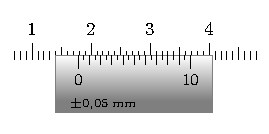
\includegraphics{_images/vernier_version_PDF_JRL_v1.pdf}
\end{center}

% ^^^^^^^^^^^^^^^^^^^^^^^^^^^^^^^^^^^^^^ %
%               Question                 %
% ^^^^^^^^^^^^^^^^^^^^^^^^^^^^^^^^^^^^^^ %

\begin{enonce}
  Que vaut le diamètre ?
\end{enonce}

\reponse{\SI{1.780\pm .050}{\milli\meter}}

\begin{corrige}
Le zéro de l'échelle mobile est entre \SI{1,7}{\milli\metre} et \SI{1,8}{\milli\metre}. Il y a 20 graduations dans l'échelle mobile, le pied à coulisse a donc une précision affichée de $\frac{\SI{1}{\milli\meter}}{20}=\SI{.05}{\milli\meter}$. La graduation qui est alignée avec une graduation fixe est la 16\ieme{} de l'échelle mobile, on lit donc 
\[
d=\SI{1,7}{\milli\metre}+16\times\SI{.05}{\milli\meter}=\SI{1.78}{\milli\meter}.
\]
Le résultat de la mesure est alors $d=\SI{1.78\pm .050}{\milli\meter}$, puisque conventionnellement les incertitudes sont données avec deux chiffres significatifs.
\end{corrige}

% ************************************** %


% ^^^^^^^^^^^^^^^^^^^^^^^^^^^^^^^^^^^^^^ %
%               Question                 %
% ^^^^^^^^^^^^^^^^^^^^^^^^^^^^^^^^^^^^^^ %

\begin{enonce}
En déduire la section droite du fil (en \si{\milli\meter\squared})
\end{enonce}

\reponse{\SI{2.49\pm 0.14}{\milli\meter\squared}}

\begin{corrige}
La section droite est un disque de diamètre $d$. Sa mesure vaut donc \(s=\pi(d/2)^2\). Numériquement on obtient 
\[
s=\pi\times \left(\frac{\SI{1.78}{\milli\meter}}{2}\right)^2
=\SI{2.4885}{\milli\meter\squared}.
\]
La section étant reliée au diamètre par une fonction puissance on a 
\[
\frac{\incertitude(s)}{s}=
2\frac{\incertitude(d)}{d}=
2\times\frac{\SI{.05}{\milli\meter}}{\SI{1.78}{\milli\meter}}=
\SI{5.6}{\percent}.
\]
Finalement, on obtient \(\incertitude(s)=\SI{0.14}{\milli\meter\squared}\) et le résultat s'écrit \(s=\SI{2.49\pm 0.14}{\milli\meter\squared}\).
\end{corrige}

% ************************************** %

% =============================================================================== %
\finEntrainement
% =============================================================================== %





% •••••••••••••••••••••••••••••••••••••••••••••••••••••••••••••••••••••••••••• %
% •••••••••••••••••••••••••••••••••••••••••••••••••••••••••••••••••••••••••••• %
\sectionFicheEntrainement{Autour du \zScore-score}
% •••••••••••••••••••••••••••••••••••••••••••••••••••••••••••••••••••••••••••• %
% •••••••••••••••••••••••••••••••••••••••••••••••••••••••••••••••••••••••••••• %

\bigskip

\begin{prerequis}
On appelle \emph{écart normalisé} (ou \emph{\zScore-score}) entre deux grandeurs $x_1$ et $x_2$,
connues avec une incertitude type $\incertitude(x_1)$ et $\incertitude(x_2)$, le nombre réel positif défini par
\[
  \zScore = \frac{|x_2 - x_1|}{\sqrt{\incertitude(x_1)^2 + \incertitude(x_2)^2}}.
\]
 
Par convention, les deux valeurs $x_1$ et $x_2$ sont dites compatibles si
$\zScore \leqslant 2$.
Comme c'est un indicateur à comparer à 2, on ne garde qu'une décimale lors de sa détermination.

\smallskip

On utilise en particulier cette définition dans le cas où une  des grandeurs, par exemple $x_1$ peut être considérée comme une référence, avec une incertitude négligeable. On a alors  \(\incertitude(x_1) \ll \incertitude(x_2)\) et la formule approchée plus simple : 
\[
\zScore = \frac{|x_2 - x_1|}{\incertitude(x_2)}.
\]
\end{prerequis}




% ********************************************************************* %
%                           ENTRAÎNEMENT                                % 
% ********************************************************************* %
% ================ Métadonnées sur l'entraînement ===================== %

\titreEntrainementFacultatif	{Z-scores et compatibilité}
\hauteurLargeurCadreReponse		{8mm}{1.6cm}
\dureeResolutionFacultative		{1} % 1, 2, 3 ou 4
\typeEntrainement				{QCM} % Newton ou QCM ou AN ou vide (exercice "normal")
\nombreColonnesQuestions		{1} % vide, 1, 2, 3, etc.
\avecPlusieursQuestions			{Y} % Y ou N
\initialisationEntrainement
% ===================================================================== %


% =============================================================================== %
\finEntrainement
% =============================================================================== %

Dans chaque situation, deux valeurs d'une même grandeur sont obtenues indépendamment. 

Indiquer, en calculant leurs \zScore-scores, si ces valeurs sont compatibles :

% ^^^^^^^^^^^^^^^^^^^^^^^^^^^^^^^^^^^^^^ %
%               Question                 %
% ^^^^^^^^^^^^^^^^^^^^^^^^^^^^^^^^^^^^^^ %

  \begin{enonce}
  La vitesse du son dans l'air est déterminée expérimentalement à \SI{349.0\pm 2.3}{\metre\per\second}. Une table de référence donne \SI{344.08\pm 0.69}{\metre\per\second}.
  \begin{listeQCM2Colonnes}
    \item Oui, elles sont compatibles
    \item Non, elles ne le sont pas
  \end{listeQCM2Colonnes}
  \end{enonce}
  
  \reponse{\reponseB{}}
  
  \begin{corrigeNewpage}
    On compare une valeur à une valeur de référence. On vérifie que l'incertitude de la valeur tabulée est très inférieure à celle de la mesure. En effet, l'inégalité
    \[
      (\SI{0.69}{\metre\per\second})^2 = \SI{0.48}{\square\metre\per\square\second} \ll (\SI{2.3}{\metre\per\second})^2 =   \SI{5.3}{\square\metre\per\square\second}
    \]
    est bien vérifiée (il y a plus d'un facteur 10 entre les deux valeurs).
    
    On peut donc utiliser la formule simplifiée : on a \(\zScore=\frac{\SI{4,92}{\metre\per\second}}{\SI{2.3}{\metre\per\second}}=\num{2.1}>2\).
    
    Ainsi, les deux valeurs sont incompatibles.
  \end{corrigeNewpage}
  
% ************************************** %


% ^^^^^^^^^^^^^^^^^^^^^^^^^^^^^^^^^^^^^^ %
%               Question                 %
% ^^^^^^^^^^^^^^^^^^^^^^^^^^^^^^^^^^^^^^ %

  \begin{enonce}
  Une température est mesurée par deux groupes en TP. Le premier groupe obtient \SI{52.900\pm 0,060}{\celsius}, le second  \SI{53.100\pm 0,060}{\celsius}. 
  \begin{listeQCM2Colonnes}
    \item Oui, elles sont compatibles
    \item Non, elles ne le sont pas
  \end{listeQCM2Colonnes}
  \end{enonce}
  
  \reponse{\reponseB{}}
  
  \begin{corrige}
    On compare deux valeurs avec la même incertitude, on doit appliquer la formule complète, mais qui se simplifie un peu puisque les incertitudes sont les mêmes. On trouve
      \[
    \zScore=\frac{\SI{.2}{\celsius}}{\sqrt{2}\times \SI{0,060}{\celsius}}=\num{2.4}>2
    \]
    
    Ainsi, les deux valeurs sont incompatibles.
  \end{corrige}
  
% ************************************** %


% ^^^^^^^^^^^^^^^^^^^^^^^^^^^^^^^^^^^^^^ %
%               Question                 %
% ^^^^^^^^^^^^^^^^^^^^^^^^^^^^^^^^^^^^^^ %

\begin{enonce}
  Une lentille est vendue pour avoir une focale de \SI{25}{\centi\metre}. Lors d'une séance de TP, cette focale est mesurée à \SI{24.05\pm ,85}{\centi\metre}.
  \begin{listeQCM2Colonnes}
    \item Oui, elles sont compatibles
    \item Non, elles ne le sont pas
  \end{listeQCM2Colonnes}
 \end{enonce} 
 
  \reponse{\reponseA{}}
  
  \begin{corrige}
    On compare une valeur à une valeur de référence exacte : on a \(\zScore=\frac{\SI{,95}{\centi\metre}}{\SI{.85}{\centi\metre}}=\num{1,1}<2\).
    D'après le critère donné, les deux valeurs sont compatibles.
  \end{corrige}
  
% ************************************** %


% =============================================================================== %
\finEntrainement
% =============================================================================== %









% ---------------------------------------------------------------------------- %
%                       Affichage des réponses mélangées                       %
% ---------------------------------------------------------------------------- %
\afficheReponsesMelangees
% ---------------------------------------------------------------------------- %

%%%%%%%%%%%%%%%%%%%%%%%%%%%%%%%%%%%%%%%%%%%%%%%%%%%%%%%%%%%%%%%%%%%%%%%%%%%%%%%%%%%%%%%%%%%%%%
\finFicheEntrainement                                                                        %
%%%%%%%%%%%%%%%%%%%%%%%%%%%%%%%%%%%%%%%%%%%%%%%%%%%%%%%%%%%%%%%%%%%%%%%%%%%%%%%%%%%%%%%%%%%%%%


% ======================================================= % 
% ============== Gestion de la compilation ============== %
% ======================================================= % 
\ifdefined\mainIsLoaded\else
\printReponsesEtCorriges
\end{document}\fi
% ======================================================= % 
% ======================================================= % 
